\section{Ablation Studies and Analysis}
\label{sec:ablation_studies}

\begin{table*}[t]
\centering
\caption{
    Ablation study on ALFWorld. 
    %
    We incrementally evaluate the contribution of turn-level intervention, teacher confidence weighting, and vanilla-scale normalization. 
    %
    Best and second-best SR among distillation methods for each setup is in \textbf{bold} and \underline{underlined}, respectively.
    % \zz{I changed \ours-NoNorm to just NoNorm, added arrows as in other tables. Also noticed that the full \ours often has the highest turn numbers, curious if there is an explanation.}
}
\vspace{-0.1in}
\label{tab:ablation_alfworld}
\setlength{\tabcolsep}{12pt}
\resizebox{\textwidth}{!}{%
\begin{tabular}{lllcccc}
\toprule
\textbf{Student Model} & \textbf{Teacher Model} & \textbf{Method}
& \textbf{Seen SR $\uparrow$} & \textbf{Seen Turns $\downarrow$}
& \textbf{Unseen SR $\uparrow$} & \textbf{Unseen Turns $\downarrow$} \\
\midrule
\multicolumn{7}{c}{\textit{Student: Qwen3-0.6B, Teacher: Qwen3-8B}} \\
\midrule
\multirow{4}{*}{Qwen3-0.6B} & \multirow{4}{*}{Qwen3-8B}
& OPD & 55.00 & 18.53 & 56.72 & 20.30 \\
& & Intervention-only & \underline{57.86} & 17.80 & \textbf{62.69} & 18.49 \\
& & NoNorm & 55.71 & 19.19 & 55.22 & 20.50 \\
& & \ours{} & \textbf{57.86} & 18.46 & \underline{61.94} & 18.89 \\
\midrule
\multicolumn{7}{c}{\textit{Student: Qwen3-1.7B, Teacher: Qwen3-8B}} \\
\midrule
\multirow{4}{*}{Qwen3-1.7B} & \multirow{4}{*}{Qwen3-8B}
& OPD & 60.00 & 17.80 & 61.94 & 17.67 \\
& & Intervention-only & 59.29 & 18.39 & \underline{66.42} & 17.68 \\
& & NoNorm & \textbf{66.43} & 17.15 & 64.93 & 18.51 \\
& & \ours{} & \underline{64.29} & 18.14 & \textbf{70.15} & 17.86 \\
\midrule
\multicolumn{7}{c}{\textit{Student: Qwen3-0.6B, Teacher: Qwen3-32B}} \\
\midrule
\multirow{4}{*}{Qwen3-0.6B} & \multirow{4}{*}{Qwen3-32B}
& OPD & 53.57 & 19.49 & 68.66 & 18.65 \\
& & Intervention-only & 53.86 & 19.21 & 67.16 & 19.40 \\
& & NoNorm & \textbf{57.86} & 19.61 & \underline{69.40} & 18.10 \\
& & \ours{} & \underline{54.29} & 19.85 & \textbf{70.90} & 17.98 \\
\midrule
\multicolumn{7}{c}{\textit{Student: Qwen3-1.7B, Teacher: Qwen3-32B}} \\
\midrule
\multirow{4}{*}{Qwen3-1.7B} & \multirow{4}{*}{Qwen3-32B}
& OPD & 58.57 & 18.89 & \underline{74.85} & 17.16 \\
& & Intervention-only & \underline{62.14} & 18.29 & \textbf{79.10} & 16.12 \\
& & NoNorm & 61.43 & 18.39 & 73.13 & 17.14 \\
& & \ours{} & \textbf{62.82} & 18.75 & 73.88 & 17.57 \\
\bottomrule
\end{tabular}%
}
\end{table*}

\begin{figure*}[t]
    \centering
    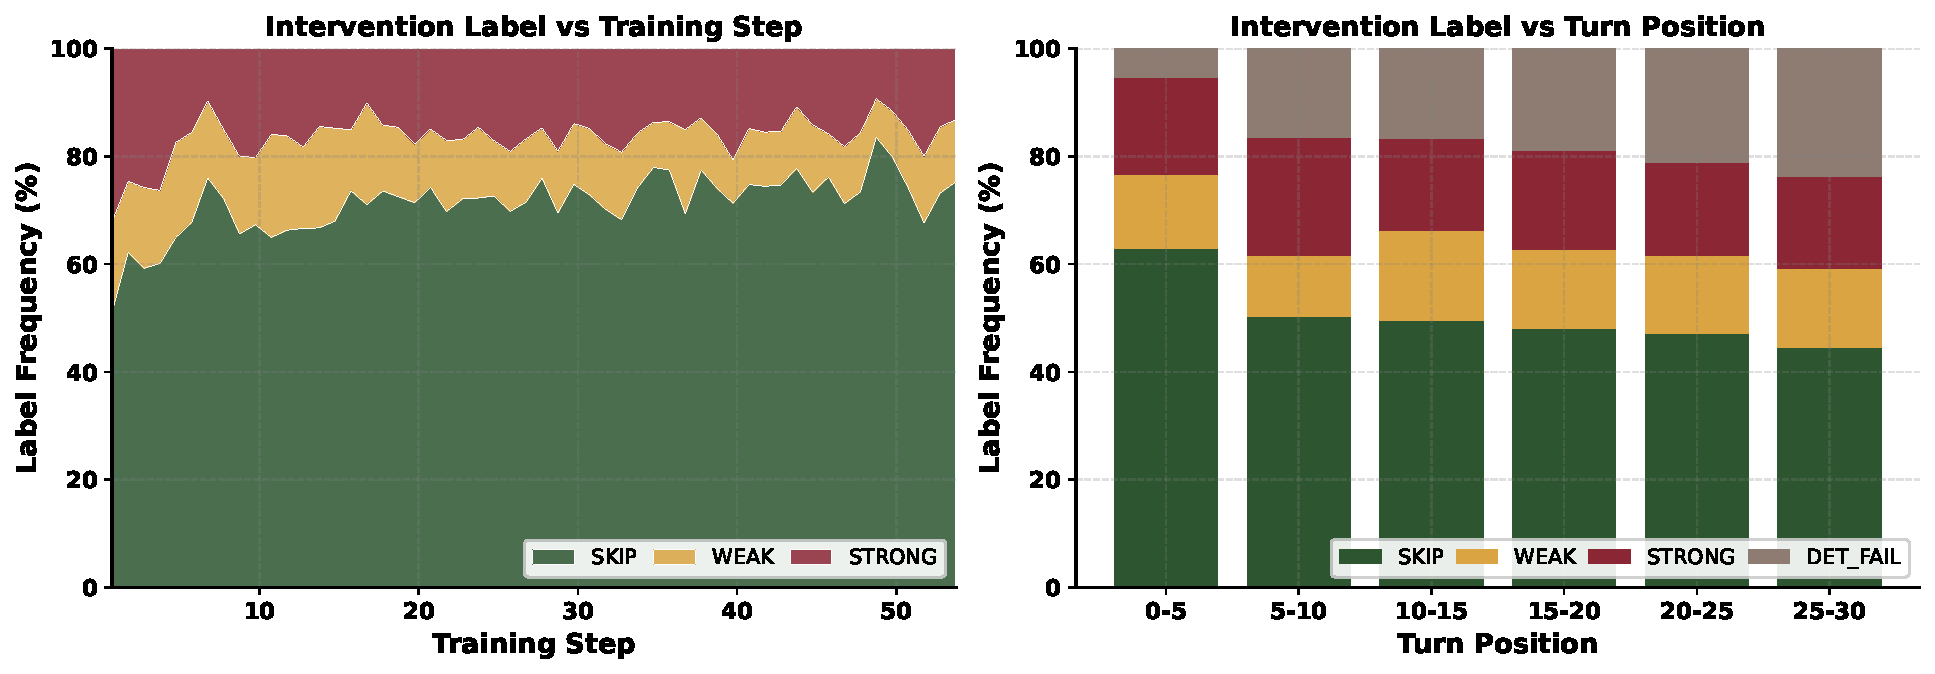
\includegraphics[width=0.9\textwidth]{figure/alfworld_slopd_intervention.pdf}
    \caption{Intervention label distribution of \ours{} on ALFWorld. Left: label frequency across training steps. Right: label frequency across turn positions. \textsc{Det-Fail} denotes deterministic failures detected before teacher intervention, such as malformed actions, failed tool calls, missing executable actions, or environment-reported execution failures.}
    \label{fig:intervention_analysis}
\end{figure*}

\subsection{Intervention Analysis}

We first analyze the intervention labels (as in \eqnref{eq:intervention_labels}) produced by \ours across training steps and turn positions. 
%
In addition to the teacher-assigned labels \textsc{Skip}, \textsc{Weak}, and \textsc{Strong}, we also report \textsc{Det-Fail}, which corresponds to the deterministic-failure short circuit described in \secref{sec:method_intervention}. 
%
These are turns where the environment or action parser provides clear negative feedback, such as malformed actions, failed tool calls, missing executable actions, or execution failures. 
%
Such turns are directly assigned full intervention without requiring additional teacher judgment.
%

As shown in \figref{fig:intervention_analysis}-\textit{left}, as training progresses, the proportion of \textsc{Skip} labels generally increases, while \textsc{Weak} and \textsc{Strong} labels decrease. 
%
This suggests that the student produces more acceptable actions over time, and the intervention mechanism correspondingly reduces unnecessary teacher supervision. 
%
The turn-position analysis (\figref{fig:intervention_analysis}-\textit{right}) shows that \textsc{Skip} remains the dominant label across the trajectory, but gradually decreases as the turn index increases. 
%
Meanwhile, \textsc{Det-Fail} becomes more frequent in later turns, indicating that response quality becomes harder to maintain as the interaction horizon grows. 
%
This aligns with the compounding-error challenge in multi-turn agents. \ours will selectively skip acceptable turns while preserving full intervention for clear execution failures, which become more frequent as interaction histories grow longer.





\subsection{Ablation Studies}

We conduct ablation studies on ALFWorld to isolate the contribution of each component in \ours.
%
We conduct an incremental comparison among three variants: \textit{Intervention-only}, which uses only the turn-level intervention weight $i_t$; \textit{NoNorm}, which further incorporates teacher confidence weighting $c_t$; and the full \ours objective, which additionally applies loss normalization.
%
As shown in \tabref{tab:ablation_alfworld}, the \textit{Intervention-only} variant already improves over this anchor in several settings, increasing unseen SR from $56.72$ to $62.69$ for Qwen3-0.6B distilled from Qwen3-8B and from $68.66$ to $79.10$ for Qwen3-1.7B distilled from Qwen3-32B.
% \zz{would it be better to add/pick a single baseline here and in the table as an anchor of comparison?}
%
This suggests that turn-level intervention labels can identify useful correction points even without requiring a task-level verifier.
%

We also notice that adding confidence weighting (the \textit{NoNorm} variant) improves some settings but can also reduce unseen generalization when the selective weights shrink the effective training signal.
%
Loss normalization addresses this issue by preserving the overall loss scale while retaining the relative turn-level weights.
%
For example, with Qwen3-1.7B distilled from Qwen3-8B, normalization improves unseen SR from $64.93$ under \textit{NoNorm} to $70.15$ under the full \ours objective; with Qwen3-0.6B distilled from Qwen3-32B, it improves unseen SR from $69.40$ to $70.90$.
%
Overall, the results show that intervention weighting, teacher confidence, and loss-scale normalization play complementary roles in selective multi-turn OPD.
%


\subsection{Sensitivity Analysis}
\label{sec:sensitivity_analysis}

\begin{table}[t]
\centering
\caption{
    Sensitivity analysis on ALFWorld using Qwen3-8B as teacher and Qwen3-1.7B as student. 
    %
    The default configuration uses $\alpha=0.5$, teacher temperature $0.0$, and standard loss normalization over all student tokens.
}
\vspace{-0.1in}
\label{tab:sensitivity}
\setlength{\tabcolsep}{20pt}
\resizebox{\textwidth}{!}{%
\begin{tabular}{llcccc}
\toprule
\textbf{Type} & \textbf{Setting}
& \textbf{Seen SR $\uparrow$} & \textbf{Seen Turns $\downarrow$}
& \textbf{Unseen SR $\uparrow$} & \textbf{Unseen Turns $\downarrow$} \\
\midrule
\multirow{4}{*}{$\alpha$}
& $0.3$ & 63.57 & 17.34 & 67.16 & 16.78 \\
& $0.5$ \;(\textit{default}) & \textbf{64.29} & 18.14 & \textbf{70.15} & 17.86 \\
& $0.7$ & 57.86 & 18.86 & 66.42 & 18.47 \\
& $1.0$ & 58.57 & 19.31 & 61.94 & 19.02 \\
\midrule
\multirow{5}{*}{Teacher temp.}
& $0.0$ \;(\textit{default}) & \textbf{64.29} & 18.14 & \textbf{70.15} & 17.86 \\
& $0.3$ & 60.00 & 18.61 & 62.69 & 18.35 \\
& $0.7$ & 60.71 & 18.77 & 65.67 & 18.34 \\
& $1.0$ & 60.71 & 18.24 & 63.43 & 18.11 \\
& $1.5$ & 57.86 & 19.24 & 63.43 & 18.74 \\
\midrule
Normalization
& All-token norm. \;(\textit{default}) & \textbf{64.29} & 18.14 & \textbf{70.15} & 17.86 \\
& Active-token norm. & 62.14 & 18.41 & 68.66 & 17.46 \\
\bottomrule
\end{tabular}%
}
\end{table}

We analyze the sensitivity of \ours in terms of teacher intervention weight $\alpha$ (as in \eqnref{eq:mapping}), teacher temperature, and normalization method, on ALFWorld using Qwen3-8B as teacher and Qwen3-1.7B as student.
%
As shown in \tabref{tab:sensitivity}, the default weak-intervention weight $\alpha=0.5$ achieves the best seen and unseen SR.
%
A smaller value, $\alpha=0.3$, remains competitive but underperforms on the unseen split, suggesting that weak interventions still provide useful supervision.
%
Larger values, such as $\alpha=0.7$ and $\alpha=1.0$, degrade performance and increase the average number of turns.
%
When $\alpha$ approaches $1$, weak interventions become similar to strong interventions, making the objective closer to standard dense OPD on ambiguous turns.
%
This suggests that ambiguous turns benefit from partial rather than full teacher correction, supporting our use of a moderate weak-intervention weight.
%

We also vary the teacher temperature used for confidence estimation.
%
The default deterministic setting, temperature $0.0$, performs the best, while higher temperatures consistently reduce success rate.
%
This is expected because the confidence score is derived from the teacher's predictive distribution, and higher temperatures can make this signal less stable for turn-level weighting.
%
Finally, we compare an alternative normalization that counts only active, non-skipped tokens in $N$ rather than all student tokens.
% \zz{Should we also add the default setting in the table? The other two types have this}
%
This variant remains competitive, reaching $68.66\%$ unseen SR, but underperforms the default vanilla-scale normalization at $70.15\%$.
%
Overall, these results support using a moderate weak-intervention weight, deterministic teacher confidence, and normalization over all student tokens as the default configuration.
%
